\chapter{Application description}\label{chapter:appdescription}

\section{Architecture}
The application will be developed using the Android Studio IDE.
The application will be developed using the Java programming language.
The application will use the Google ARCore framework\cite{ARCore}.
The application will use the Firebase cloud database to store the models. The application will use the \ac{QR} code reader to import the models.
The application will use the Google Vision API to recognize the \ac{QR} code.
As shown in Figure \ref{fig:architecture}, the architecture of the application consists of...

\begin{figure}[ht]
    \centering
    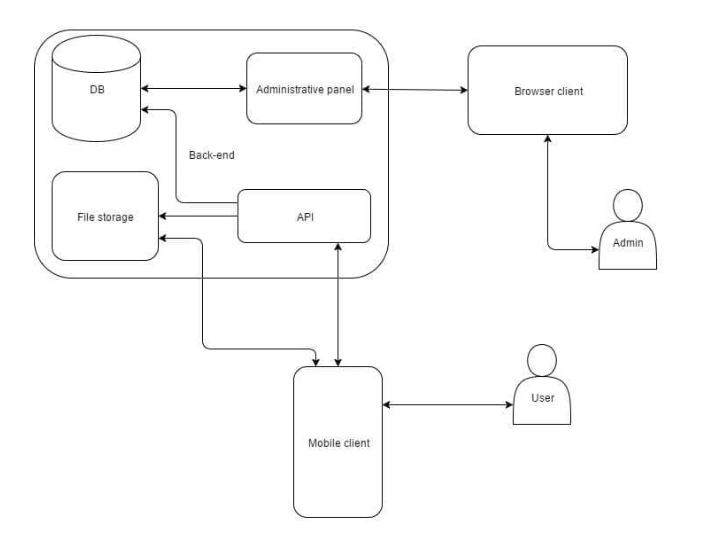
\includegraphics[width=1\textwidth]{img/architecture.png}
    \caption{Architecture}
    \label{fig:architecture}
\end{figure}

\begin{itemize}
    \item \textbf{Android Version 7.0+} - to use the application on the phone
    \item \textbf{Android Studio} - IDE for Android development
    \item \textbf{Firebase} - Cloud DataBase for where the models will be retrieved
    \item \textbf{Java} - Programming language
    \item \textbf{Google ARCore} - \ac{AR} framework
\end{itemize}

\clearpage

\section{Diagrams}
\subsection*{Class Diagram}
As shown in Figure \ref{fig:ClassDiagram}, the class diagram of the application consists of the following main classes: MainActivity, QRActivity and LibraryActivity.

The MainActivity class is the main class of the application. It is the first class called when the application is started, and it is responsible for the \ac{AR} mode. It contains methods dedicated to interacting with the \ac{3D} models (moving the model, rotating the model, scaling the model).

The QRActivity class is responsible for the \ac{QR} code reader. It has a method called when a \ac{QR} code is scanned and verifies if it is valid. It will check if the model is already imported. If the model is already imported, it will load it from the local storage; it will also request the Google Bucket Storage.

Lastly, the LibraryActivity class is responsible for the list of models and the loading of the models.
\begin{figure}[ht]
    \centering
    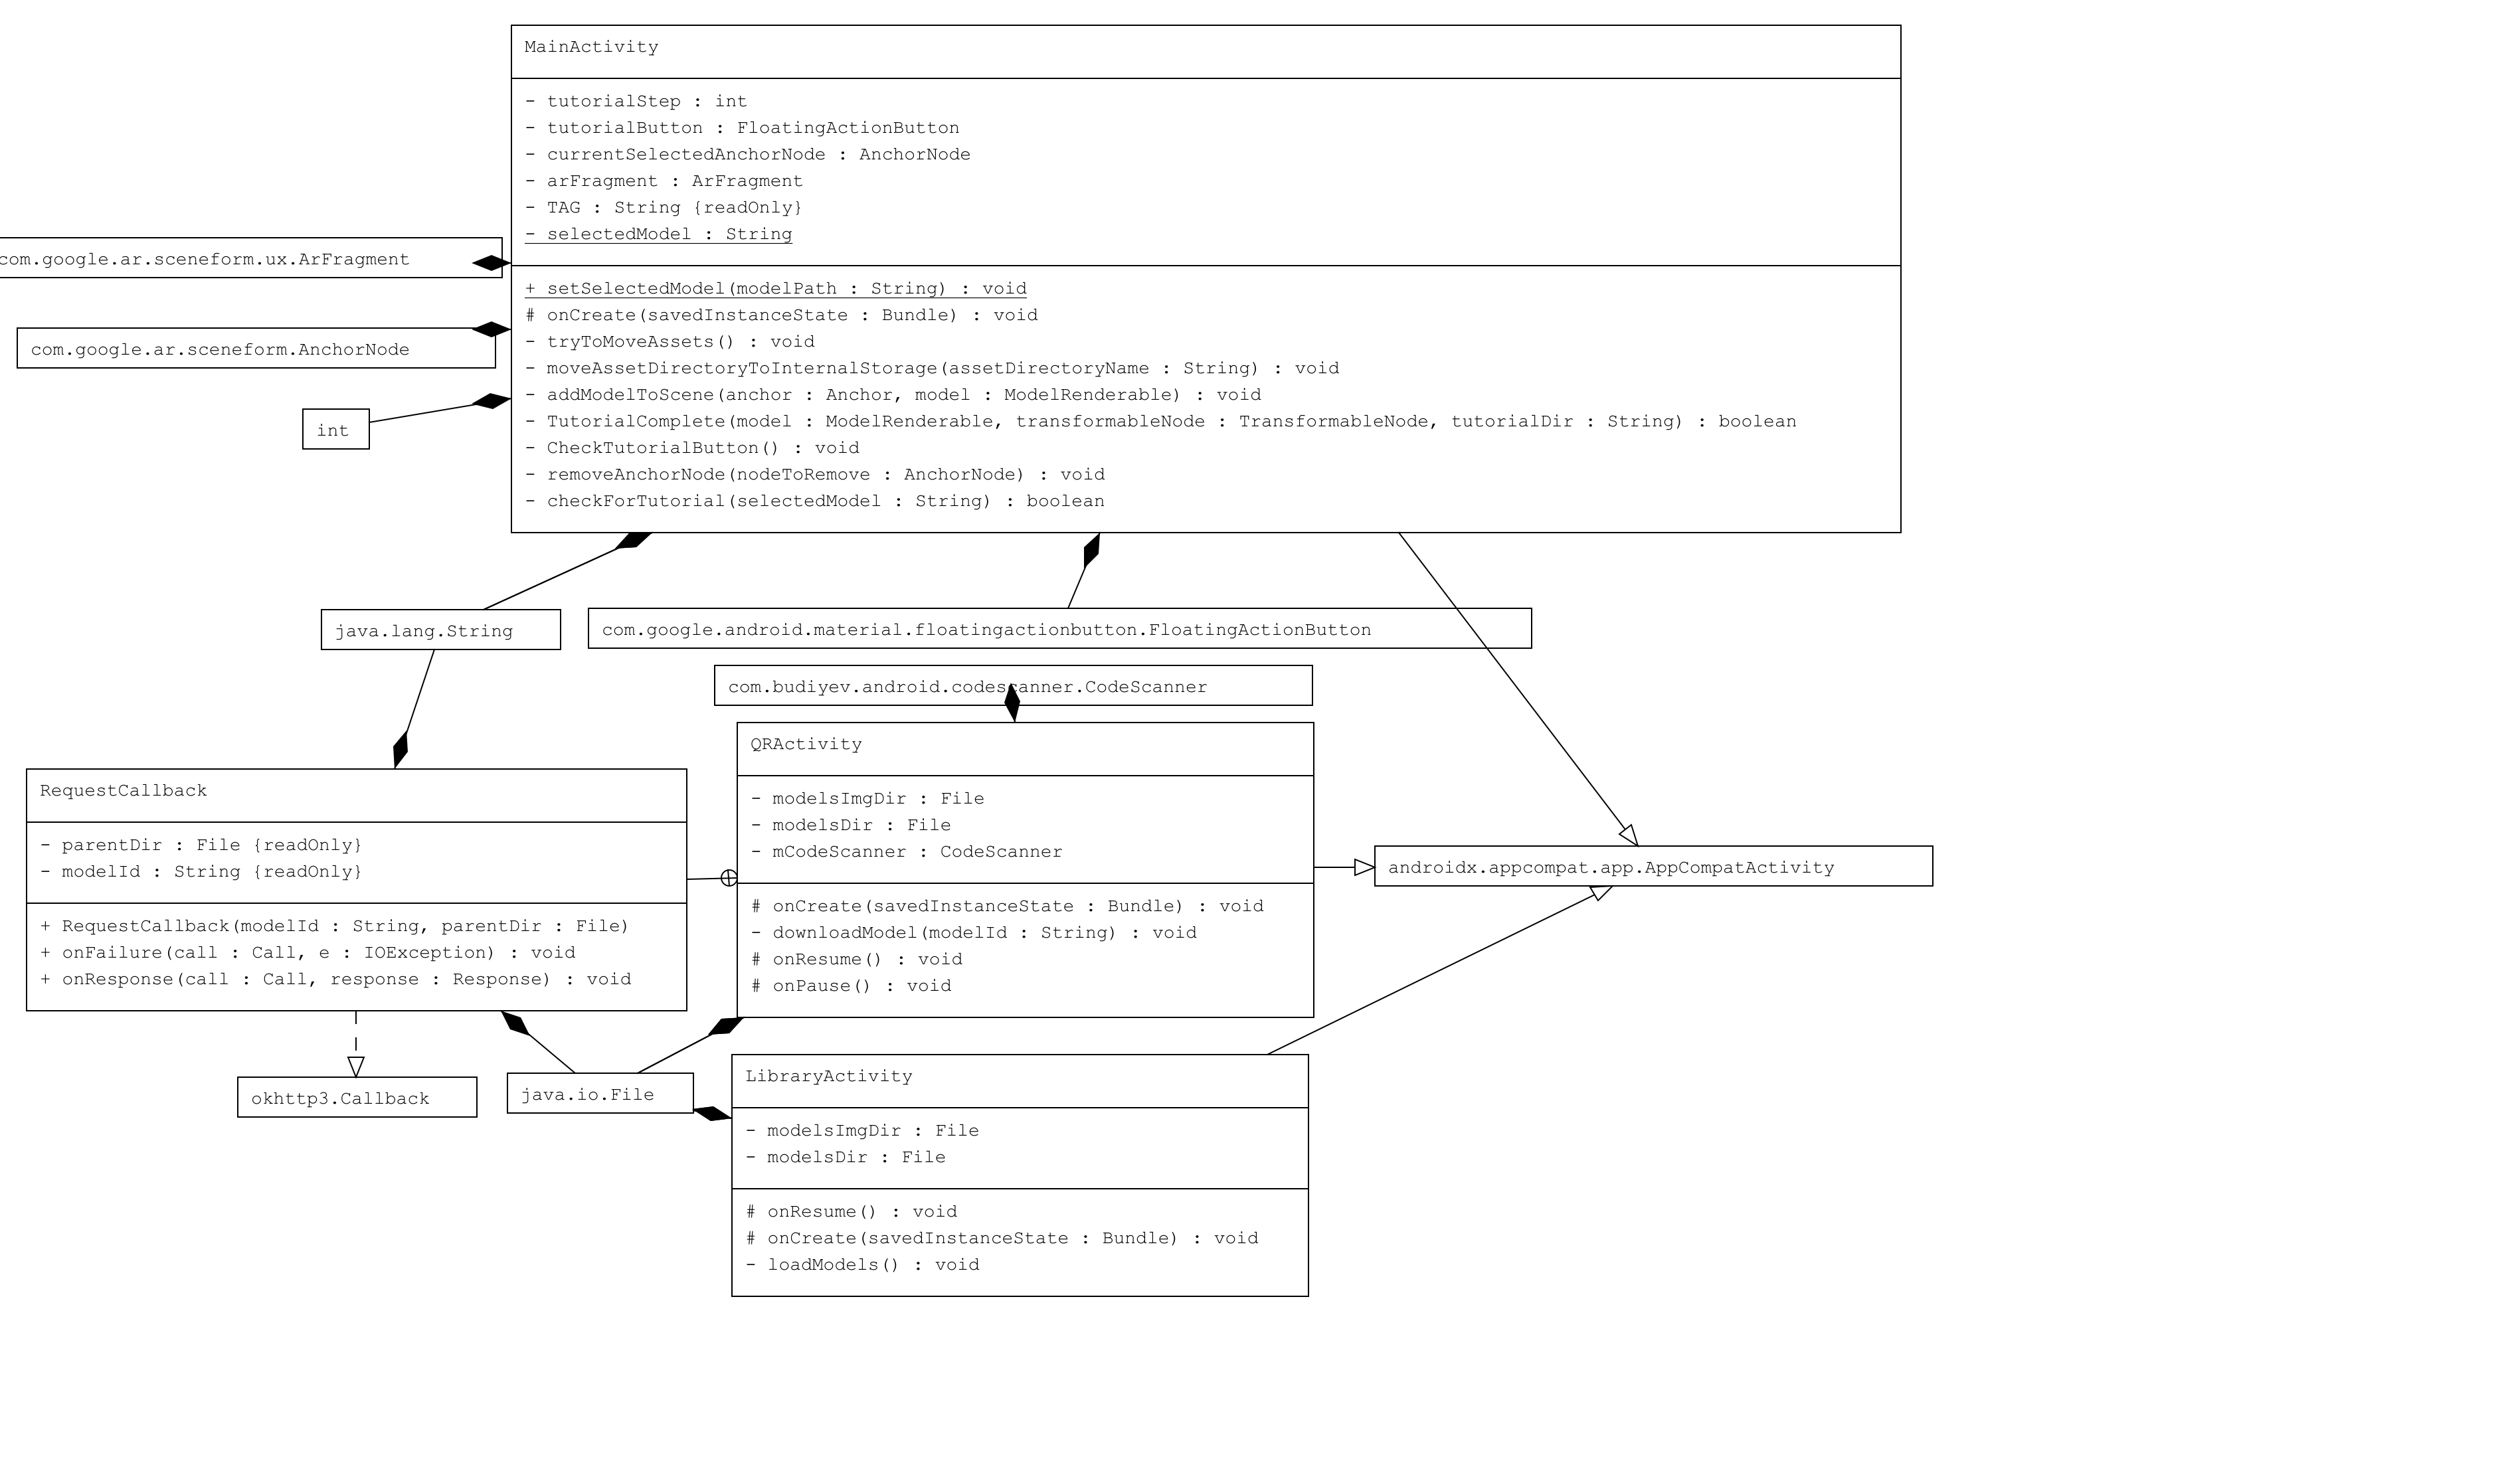
\includegraphics[height=0.9\textwidth]{img/ClassDiagram.png}
    \caption{Class Diagram}
    \label{fig:ClassDiagram}
\end{figure}


\subsection*{Use Case Diagram}
By looking at the Use Case Diagram in Figure \ref{fig:UseCaseDiagram}, we can see what the user is able to do inside the application. RealityEnhance allows the users to scan a \ac{QR} code load or to import a new model. It also gives users the power to interact with the \ac{3D} models in the \ac{AR} mode. The users can also browse a library of already imported models.

The ability to interact with the \ac{3D} models is a very important feature of the application. It allows the users to see the models from different angles and to change the size, orientation and position using familiar gestures. It also gives users the possibility to remove a selected model that is already placed in the \ac{AR} scene.
\begin{figure}[ht]
    \centering
    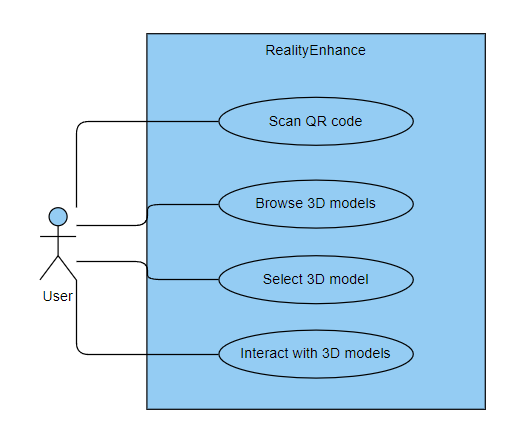
\includegraphics{img/UseCaseDiagram.png}
    \caption{Use Case Diagram}
    \label{fig:UseCaseDiagram}
\end{figure}

\clearpage

\subsection*{Sequence Diagram}
The Sequence Diagram in Figure \ref{fig:SequenceDiagram} shows the interaction between the user and the application. The user starts the application and is presented with a prompt that will request permission to use the camera. After that, the \ac{AR} module will begin to scan the user's surroundings in order to map the environment. For importing a new model, RealityEnhance uses a \ac{QR} code scanner that will check if the code is valid.
\begin{figure}[ht]
    \centering
    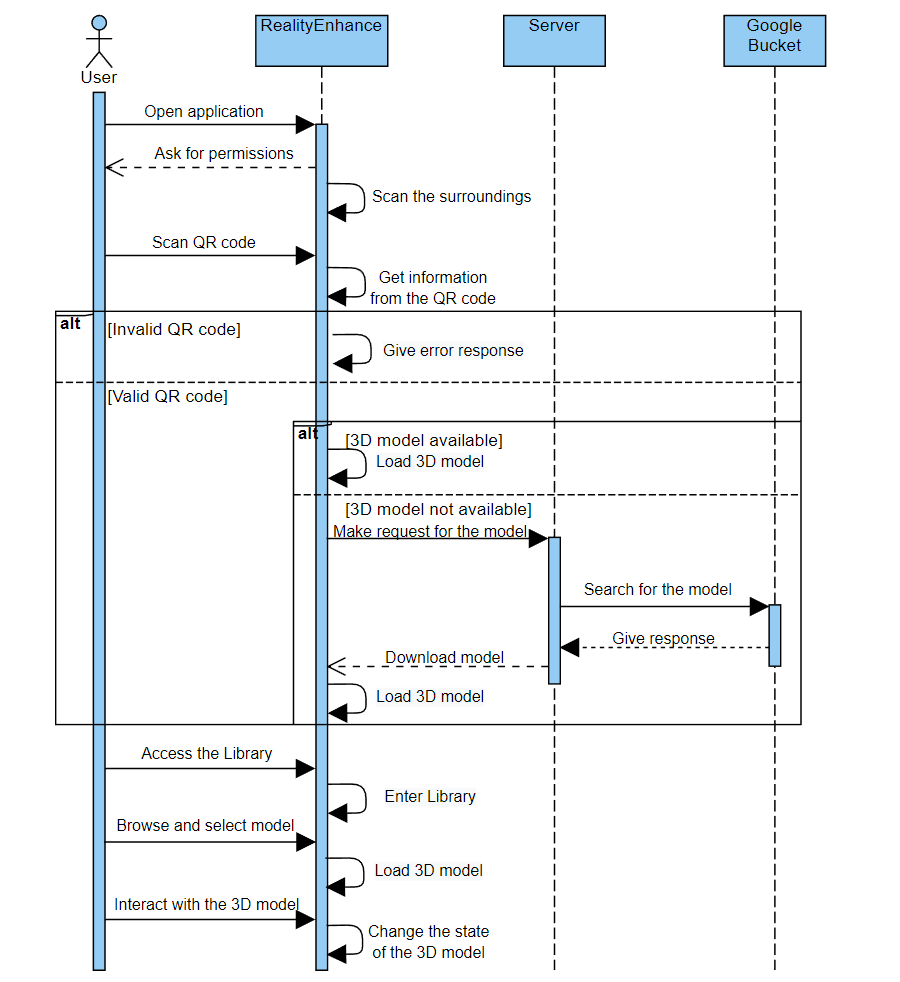
\includegraphics[width=1\textwidth]{img/SequenceDiagram.png}
    \caption{Sequence diagram}
    \label{fig:SequenceDiagram}
\end{figure}

If the code fails the validation process, the user will be notified and will be prompted to scan another code. If the code is valid, the application will check if the model is already in the local storage, and it will load it. If the model is not in the local storage, the application will make a request to Google Bucket Storage to retrieve all the information about the model (model file, textures, model image, model guide/interactive guide). After the request is completed, a response will be sent back with all the information about the model. The model will then be saved in the local storage and loaded in the \ac{AR} scene.

The user can also browse the Library of already imported models. It also has access to the \ac{QR} scanner interface and can search for the desired model that is wanted to be loaded in the \ac{AR} scene.

The interaction between the user and the model bridges the virtual-physical gap and helps build a sense of immersion.

\clearpage

\section{Implementation}
Implementation details...

\section{Deployment}
Deployment details...
